\section{Module 4. Non-stationary noise filtering 1}

The objective of fourth module is to remove Rician noise from MR images. If
both real and imaginary parts of signal are corrupted with zero-mean
uncorrelated Gaussian noise with equal variance, the envelope of magnitude
signal will follow a Rician distribution. Many processes allow to
remove noise, here the method is used to denoise MR images is the
linear minimum square error estimator (LMMSE). The main purpose of
LMMSE is to find a closed-form estimator for a signal that follows
a Rician distributions. It is more efficient than optimization-based
solutions. The estimator uses information of the sample distribution of local statistics of the image such as the local mean, the local variance and the local mean square value. In this method, the true
value for each noisy pixel is estimated by a set of pixels selected from a local neighborhood.

\hfill{}\\
\textbf{The LMMSE estimator}\\

Scalar parameter $\theta$ is to be estimated based on the data set $\{x[0],x[1], ... , x[N - 1]\}$. The unknown parameter is modeled as the realization of a random variable. We assume only a knowledge of the first two moments. $\theta$ may be estimated from x is due to the assumed statistical dependence of 0 on x as summarized by the joint PDF p(x, B), and in particular, for a linear estimator we rely on the correlation between $\theta$ and x. We now consider the class of all linear estimators of the form:

\begin{equation}
\begin{aligned}\widehat{\theta}=\sum\limits_{n=0}^{N-1} a_nx[n]+a_N \end{aligned}
\label{m4eq0}
\end{equation}

and choose the weighting coefficients $a_n$'s to minimize the Bayesin MSE (mean square error):

\begin{equation}
\begin{aligned}Bmse(\widehat{\theta})=E[(\theta - \widehat{\theta})^2] \end{aligned}
\label{m4eq1-1}
\end{equation}
where the expectation is with respect to the PDF p(x,O). The resultant estimator is
termed the linear minimum mean square error (LMMSE) estimator.

\begin{figure}[H]
\centering{}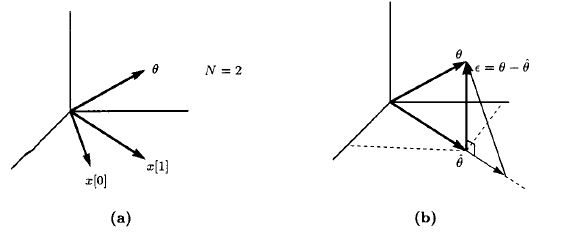
\includegraphics[scale=0.7]{figures/Module_4/LMMSE-estimator}\caption{Geometrical interpretation of LMMSE estimator} \label{fig:figures/Module_4/LMMSE-estimator}
\end{figure}


The LMMSE estimator admits a geometrical interpretation, the random variables $\theta$, $x[0], x[1], ... , x[N - 1]$ as elements in a vector space as shown symbolically in Fig. \ref{fig:figures/Module_4/LMMSE-estimator}a. This approach is useful for conceptualization of the LMMSE estimation process. As before, we assume that
\begin{equation}
\begin{aligned}\widehat{\theta}=\sum\limits_{n=0}^{N-1} a_nx[n] \end{aligned}
\label{m4eq1-2}
\end{equation}
where $a_N$ = 0 due to the zero mean assumption. The weighting coefficients an should be chosen to minimize the MSE:
\begin{equation}
\begin{aligned}E[(\theta - \widehat{\theta}^2]= E[(\theta-\sum\limits_{n=0}^{N-1} a_nx[n])^2]\end{aligned}
\label{m4eq1-1}
\end{equation}

But this means that minimization of the MSE is equivalent to a minimization of the squared length of the error vector $\epsilon$ = $\theta$ - $\widehat{\theta}$. The error vector is shown in Fig. \ref{fig:figures/Module_4/LMMSE-estimator}b for several candidate estimates. Clearly, the length of the error vector is minimized when $\epsilon$ is orthogonal to the subspace spanned by $\{x[0], x[1], ... , x[N - 1]\}$.

\hfill{}\\
\textbf{The LMMSE estimator for MR image}\\

The LMMSE estimator for a 2-D signal with Rician distribution is defined:

\begin{equation}
\begin{aligned}\widehat{A_{ij}^{2}}=E\{A_{ij}^{2}\}+C_{A_{ij}^{2}M_{ij}^{2}}C_{M_{ij}^{2}M_{ij}^{2}}^{-1}(M_{ij}^{2}-E\{M_{ij}^{2}\})\end{aligned}
\label{m4eq1}
\end{equation}
where $A_{ij}$ is the unknown intensity value in pixel $ij$, $M_{i}j$
the observation vector, $C_{A_{ij}^{2}M_{ij}^{2}}$ the cross-covarience
vector and $C_{M_{ij}^{2}M_{ij}^{2}}$ the covarience matrix. If the
estimator is simplified to be pointwise, vectors and matrics become
scalar values. 
To calculate the second order moment we assume local ergodicity, the expectation ($E\{\}$) may be replaced by sample estimator, that can be defined: 
\begin{equation}
\begin{aligned}\langle I_{ij}\rangle=\frac{1}{|\eta_{ij}|}\sum\limits_{p\epsilon\eta_{ij}} I_p \end{aligned}
\label{m4eq2}
\end{equation}
with $\eta_{ij}$ a square nighbourhood around the pixel $ij$. The finally equation for LMMSE is defined:
\begin{equation}
\begin{aligned}\widehat{A_{ij}^{2}}=\langle M_{i}j^{2}\rangle-2\sigma_{n}^{2}+K_{ij}(M_{ij}^{2}-\langle M_{ij}^{2}\rangle)\end{aligned}
\label{m4eq3}
\end{equation}
with $K_{ij}$ 
\begin{equation}
\begin{aligned}K_{ij}^{2}=1-\frac{4\sigma_{n}^{2}(\langle M_{i}j^{2}\rangle-2\sigma_{n}^{2})}{\langle M_{i}j^{4}\rangle-{\langle M_{i}j^{2}\rangle}^{2}}\end{aligned}
\label{m4eq4}
\end{equation}

The estimated noise is needed to use the LMMSE filter. The map of noise is prepered one module before. The use of the LMMSE method should makes the filtering process computationally far more efficient and easier to implement. 

\hfill{}\\
\textbf{Module I/O}\\
\textbf{\emph{Module input}}: Reconstructed, normalized and corrected data, noise maps.
\textbf{\emph{Module output}}: Images without Rician noise.
